\graphicspath{{chapters/01/}}
\chapter{Introduction}

\section{Genetics vs Genomics}

	\subsection{Genetics}
	Genetics is the study of heredity, or how the characteristics of living organisms are transmitted from one generation to the next via DNA.
	It dates back to Augustinian friar and scientist Gregor Mendel.
	It involves the study of a specific and limited number of genes or their part that have a known function.

	\subsection{Genomics}
	Genomics is the study of the entirety of an organism's genes, the genome.
	Using high-performance computing and math techniques known as bioinformatics, genomics researchers analyse enormous amounts of DNA-sequence data to find variations that affect health, disease or drug response.
	In human that means searching through about $3$ billion units of DNA across $23000$ genes.

	\subsection{Differences}
	The main difference between genomics and genetics is that genetics scrutinizes the functioning and composition of the single gene, where genomics addressees all genes and their relationships in order to identify their combined influence on the growth and development of the organism.

	\subsection{Role of computational biology}
	Computational biology offer a wide range of numerical methods to analyse and integrate large scale data towards the understanding of molecular, cellular and structural biology.
	The focus of this course is on human genomics and how to mine raw data, how to exploit it for quality control and how to interpret the results in the context of human disease, especially cancer.

\section{Human Genomics - the Basis}
\subsection{Genetic Make-Up}
The individual's genetic make-up is different in all of us and it is responsible for human diversity.
SNPs (single nucleotide polymorphisms) and CNVs (copy number variants) contribute to make us all different. 
The majority of external phenotypes are from genetic variance that we inherit (but they can also be aquired). 

		\subsubsection{Single nucleotide polymorphisms}
		Single nucleotide polymorphisms or SNPs are changes of one nucleotide in the sequence of a gene.
		They constitute $1\%$ of the difference between two unrelated individuals' genomes.

		\subsubsection{Copy number variants}
		Copy number variants or CNVs are difference of the number of allele for a gene present in one individual.
		They contribute much more than SNPs in the difference between unrelated individuals.
		If both parents are monozygous in one gene the child could have zero copy of the gene.

\subsection{Inherited variants' relevance}
Inherited variants can be characterized by penetrance and allele frequency.

\begin{figure}[htbp!]
    \centering
    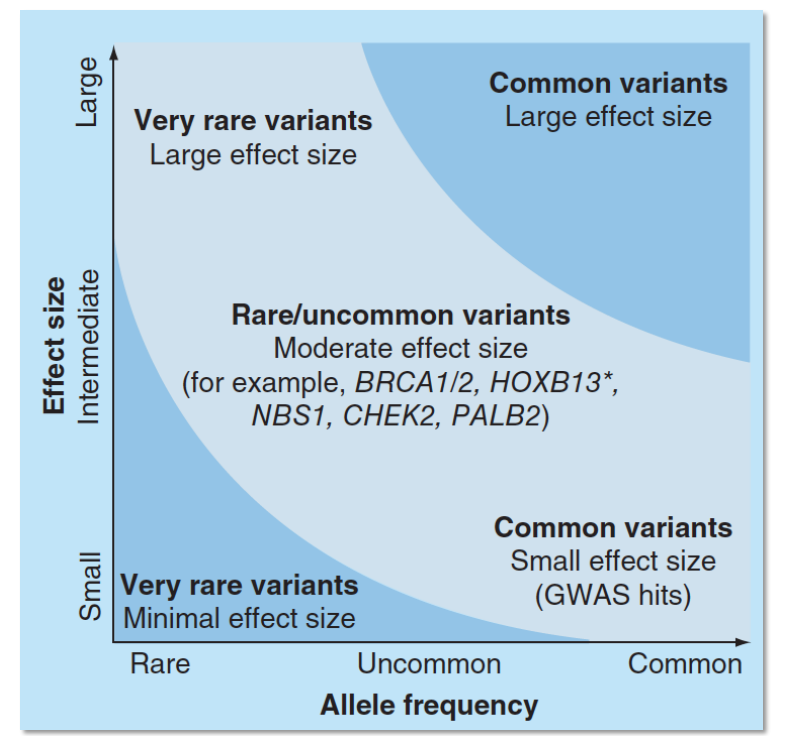
\includegraphics[width=0.5\textwidth]{relevance.png}
    \caption{R. Eeles, Future Sci. OA (2016) 2(1), FSO87. Review on prostate cancer}
    \label{fig:relevance}
\end{figure}

\paragraph{Penetrance}
Penetrance is the proportion of individuals carrying an allele (or genotype) that also expresses the trait (or phenotype) associated with it.

\paragraph{Allele frequency}
Allele frequency is the ratio between the number of times the allele of interest is observed in a population over the total number of copies of all the alleles at that particular genetic locus in the population.
			
Recent studies have shown that genetic variance contributes to predisposition to certain deseases. 
What is also emerging is that if we are dealing with a very rare variant, if this variant is pathogenic, it haso also high penetrance.
Meaning, if the variant is pathogenic and very rare, it's very probable that all patients affected by the desease carry this mutation. This is shown in the top part of the diagram shown in figure \ref{fig:relevance}.
On the other hand, common variants could be associated to predisposition or susceptability to the deasese, but the penetrance is very low. 
In the middle on the diagram we find very well-known variants correlated to cancer. The majority of these have a moderate size effect (not everyone who has the variation develops the desease).

\subsection{Differences in Genetic Make-Up, an example}
One example of how the genetic make-up plays a role in deases is the ADME genes. 
ADME stands for \textit{Absorption, distribution, metabolism and elimination}. 
It is a set of genetic variants that are able to change ability of the organism to react to certain compounds (pharmacokinetic variability),influencing the patients’ treatment response.
Both common and rare variants are involved.
A therapeutic approach that considers these variations could be very useful in precision medicine.

Somatic variance: not acquired from parents. SNV and SNP are basically the same thing, but SNV are restricted to a certain population of cells, while SNP are genetically encoded in all cells of the organism. Other types of somatic variance are rearrangemets (gene translocation, chromosome breakage, chromotripsy), somatic copy number changes are equivalt to copy number variance but somatic (SCNA). 

\subsection{Acquired DNA aberrations}
Variants that are not inherited from parents and are not transmitted to offspring are called \textbf{somatic variants}. 
They are usually caused by DNA aberrations.
DNA aberrations happen in diseased or aged cells and are the key to cancer genomics.
They can be 
\begin{itemize}
\item  Single nucleotide variants (or SNV or point mutation). SNV and SNP are basically the same thing, but SNV are restricted to a certain population of cells, while SNP are genetically encoded in all cells of the organism.
\item Indels or deletions
\item Rearrangements
\item Somatic copy number aberrations or SCNA
\end{itemize}

		\subsubsection{Types of acquired DNA aberrations} \label{subsec:aberrations}
		

			\paragraph{Translocation}
			Translocation happens when a sequence is moved from one genetic locus to another.
			It can be a balanced translocation, meaning that the overall quantity of DNA is maintained (two sequences exchange locus), or unbalanced, where only one sequence move (insertion) 

			\paragraph{Inversion}
			Inversion happens when a sequence inverts its orientation. It involves only one 		chromosome.
			Importantly, in the sequence of the inversion nothing changes, the change will be detected only at the head and tail of the inversion.
Copy number changes (DNA quantity): duplication and dletion. COuld involve one or more chromosomes

			\paragraph{Copy number changes}
			It refers to a change in the quantity of DNA. 
			In duplication a sequence doubles its copy number.
			In deletion a sequence is lost.

			\paragraph{Chromoplexy}
			From the Greek \textit{pleko}, meaning to weave, or to braid.
A class of complex somatic DNA rearrangements whereby abundant DNA deletions
and intra- and inter-chromosomal translocations that have originated in an
interdependent way occur within a single cell cycle. 

			\paragraph{Chromothripsis}
			(From the Greek \textit{thripsis}, meaning shattering into pieces).
A clustered chromosomal rearrangement in confined genomic regions that results
from a single catastrophic event, usually limited to one chromosome. 
			\paragraph{Kataegis}
			 (From the Greek kataigis, meaning thunder).
A phenomenon that is characterized by large clusters of mutations (hypermutation) in
the genome of cancer cells. An APOBEC family enzyme might be responsible for the
kataegis process.

\footnote{See  Khurana E et al, NATURE REVIEWS | GENETICS, 2016 }


\section{Experimental techniques to detect variants/aberrations}
\subsection{Cariotyping}
Basically all the aberrations described in \ref{subsec:aberrations} were discovered in the last 10-15 years because there's the need of NGS. 
Cariotyping indeed is not enough! 
Sequence specific variants, breakpoints, etc. could not be detected until NGS. 

\section{Sequence capture for cancer genomics}
In the paper \footnote{Meyerson et al., Nature Reviews Genetics 2010} it is described a typical sequence capture for cancer genomics. 
One of the main realizations is that the test reference genome is the normal (non-cancer) DNA. 
Intuitively, we align both cancer and normal DNA so that we can detect if an aberration is cancer specific or it is present also in the normal DNA. 
The \textbf{match normal} is used to distinguish SNV from rare SNPs, but also copy number variation. 
Baits are nowadays used in the sequencing step, in order to sequence only the exome (usually, money issue). 
Another concept is the need to sequence \textit{deeply}, to find subclonal events that give the cancer maybe some fitness (escaping immune system), but also because if the sample comes from the tissue, there are both cancer and some healthy cells and we need to able to distinguish them.
A more in depth discussion is provided in *paper*.

\subsection{Single End (SE) and Paired End (PE) reads}
Paired end useful especially for detecting structural variance. Massive information of relative position of a molecule wrt the reference gneome.

\begin{figure}[htbp!]
    \centering
    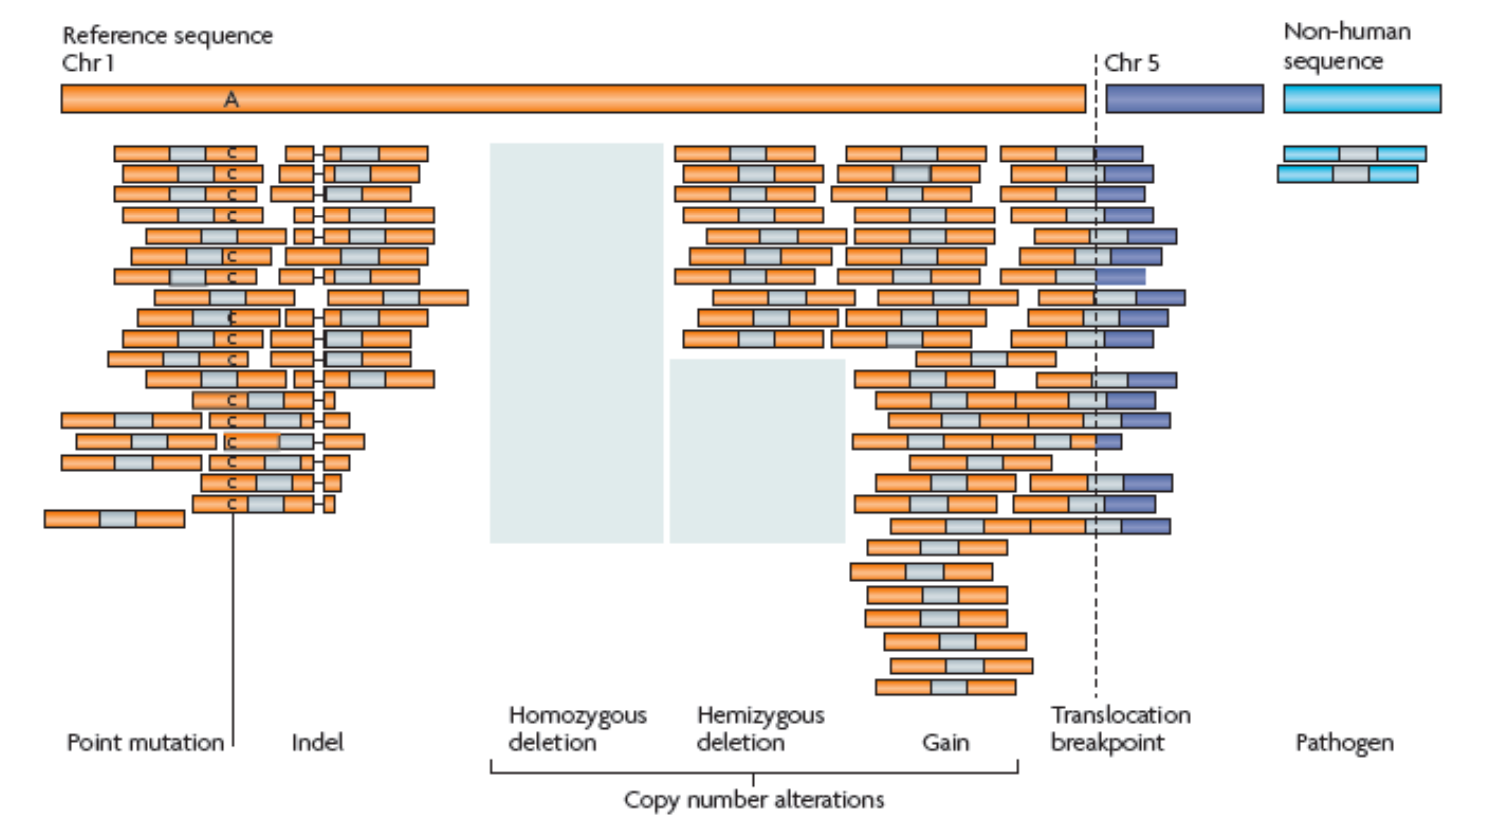
\includegraphics[width=0.7\textwidth]{igv.png}
    \caption{\textit{Advances in understanding cancer genomes through second-generation sequencing}, Meyerson et al., Nature Reviews Genetics 2010}
    \label{fig:igv}
\end{figure}

Figure \ref{fig:igv} gives a nice graphical overview of genomic aberrations detectable by NGS, especially using PE sequencing. 
Important to notice is that performing PE sequencing is like having double the coverage. 
Both for homozygous and hemizygous deletions and insertions the single most important thing we need to care about is to have enough coverage on the whole experiment to perform significative downstream analysis. 
An important thing to notice in \ref{fig:igv} is the translocation breakpoint: without PE we would not be able to detect the translocation event. 

 















